\documentclass[pdftex,12pt,a4paper]{report}

\usepackage[pdftex]{graphicx}
\usepackage[ansinew]{inputenc}
\usepackage{geometry}
\usepackage{bbold}
\usepackage{program}
\usepackage[toc,page]{appendix}
\usepackage{subcaption}
\usepackage{url}
\usepackage{textcomp}
\usepackage{gensymb}
% float forces latex to place image right "HERE"
\usepackage{float}
% math utility package
%\usepackage{mathtools}
\usepackage{savesym}
\savesymbol{implies}
\savesymbol{overset}
\usepackage{amsmath}
\savesymbol{lneq}
\usepackage{amssymb}
\geometry{a4paper,left=2.5cm,right=2.5cm, top=2.5cm, bottom=3cm}
\newcommand{\HRule}{\rule{\linewidth}{0.5mm}}

% declare macros
%\DeclarePairedDelimiter\ceil{\lceil}{\rceil}
%\DeclarePairedDelimiter\floor{\lfloor}{\rfloor}

% definition for ToC

\usepackage{lipsum}% http://ctan.org/pkg/lipsum
\usepackage{titletoc}% http://ctan.org/pkg/titletoc
\titlecontents*{chapter}% <section-type>
  [0pt]% <left>
  {}% <above-code>
  {\bfseries\chaptername\ \thecontentslabel\quad}% <numbered-entry-format>
  {}% <numberless-entry-format>
  {\bfseries\hfill\contentspage}% <filler-page-format>

\begin{document}
\begin{titlepage}

%%LR
\sffamily

\begin{center}


% Oberer Teil der Titelseite:

\includegraphics[width=0.3\textwidth]{logo2.jpg}
\hfill

\includegraphics[width=0.4\textwidth]{logo1.jpg}  
\\[5cm]

{\Large Department of Mathematics}\\[0.5cm]
{\Large Chair of Mathematical Modeling of Biological Systems}\\[0.5cm]
{Technische Universit\"at M\"unchen}\\[2cm]
{\Large Master's Thesis in Bioinformatics}\\[1.5cm]

% Title
\HRule \\[0.4cm]
{ \huge \bfseries Single-cell analysis of cancer drug response using computer vision and learning algorithms on time-lapse micro-trench data}\\[0.4cm]

\HRule \\[1.5cm]

{\Large Pandu Raharja}\\[2.5cm]

\vfill
\end{center}
\end{titlepage}
%% THIS REMOVES PAGE NUMBER
%%\pagestyle{empty}

%%LR comprehensive title
\begin{titlepage}
{\sffamily


\begin{center}

\includegraphics[width=0.3\textwidth]{logo2.jpg}
\hfill

\includegraphics[width=0.4\textwidth]{logo1.jpg}  
\\[1.5cm]  

{\Large Department of Mathematics}\\[0.5cm]
{\Large Chair of Mathematical Modeling of Biological Systems}\\[0.5cm]
{Technische Universit\"at M\"unchen}\\[1cm]

{\Large Master's Thesis in Bioinformatics}\\[2cm]
{\textbf{\Large Single-cell analysis of cancer drug response using computer vision and learning algorithms on time-lapse micro-trench data}}\\[2cm]
{\textbf{\Large Wirkungsanalyse von Krebsmedikamenten in Einzeller Aufl\"osung durch die Anwendung von Computer-Vision- und Machine-Learning-Algorithmen auf Microtrench- Videoaufnahme}}\\[4cm]

\end{center}
\begin{center}\Large
  \begin{tabular}{ll}
    Author:& Pandu Raharja\\
    Supervisor: &  Prof. Dr. Fabian Theis, Dr. Carsten Marr\\
    Advisor:        &  Prof. Dr. Fabian Theis\\
    & Prof. Dr. Dmitrij Frishman\\
    Submitted:     &  15.12.2017
  \end{tabular}
\end{center}

}% end title page

\end{titlepage}


%%%%%%%%%%%%%%%%%%%%%%%%%%%%%%%%%
% thesis content starts here
%%%%%%%%%%%%%%%%%%%%%%%%%%%%%%%%%

{\parindent 0cm
%%%%%%%%%%%%%%%%%%%%%%%%%%deutsche Version%%%%%%%%%%%%%%%%%%%%%%%%%%%%%%
  
  \section*{Selbst\"andigkeitserkl\"arung}
  Ich erkl\"are hiermit, dass ich die vorliegende Arbeit selbst\"andig verfasst 
  und nur unter Verwendung der angegebenen Quellen und Hilfsmittel angefertigt habe. 
  Weiterhin erkl\"are ich, eine Diplomarbeit in diesem Studiengebiet erstmalig einzureichen.\\
  \vspace{3\baselineskip}
  
  M\"unchen, den \today \hspace{0.1\linewidth}\parbox{0.3\linewidth}{\dotfill}

%%%%%%%%%%%%%%%%%%%%%%%%%%englische Version%%%%%%%%%%%%%%%%%%%%%%%%%%%%%%%%%%%%%%%%%%%%%%%%%%%%%%%%%

\section*{Statement of authorship}
I declare that I completed this thesis on my own and that information which has been 
directly or indirectly taken from other sources has been noted as such. Neither this 
nor a similar work has been presented to an examination committee.

  \vspace{3\baselineskip}
  
  Munich, \today \hspace{0.1\linewidth}\parbox{0.3\linewidth}{\dotfill}
}

\newpage

\chapter*{Acknowledgement}

First and foremost, I would like to thank mom and dad, for the support even from faraway lands. Even though we are continents apart, your pray and hope will be always with me.\\

To Jennifer Carissa, whose support has made it possible to go through the hard parts of my life in the last years. This thesis is only possible because of you.\\

To Julian, Ganesh and other best friends which I resort to for personal assistance. Friends really are hard to find.\\

And finally, to Prof. Fabian Theis, Prof. Joachim R\"adler, Elisavet Chatzopoulou, Felix Buggenthin and Alexandra Murschhauser for tremendous assistant in doing this project. Never did I know a project could be done in this maner.\\

Finally for my best supervisor, Carste Marr. Your boundless patience, deep insight and attention to detail have made this project impossible without your selfless assistance. I hope we could do more things in the future. 

\newpage

\chapter*{Terminology and abbreviations}

{
\flushleft

Following terms are used frequently in this thesis and therefore merit special explanation:

\begin{tabular}{ l l }
\textbf{Name} & \textbf{Explanation} \\
micro-trench & Single unit of micro-trench inside a well \\
wafer & The plate where the microtrench is manufactured on\\
slice & An image \\
stack & An ordered sequence of images (usually coming from the same channel) \\
channel & A connection between data source (camera) and storage. Images coming\\
 & from the same channel have same capture properties formatting.
\end{tabular}

\vspace{5mm}

Note that in this thesis, following things are used interchangeably:

\begin{itemize}
\item image and slice, while referring to an image particularly a capture image of the trenches and its processed versions.
\item image and figure, while referring to an image shown in this paper in general.
\end{itemize}



\vspace{5mm}

\begin{tabular}{ l l }
\textbf{Symbol} & \textbf{Explanation} \\
$M$ & A stack of images \\
$M_t$ & An image captured at time t (t-th image) \\
$M_{t, x, y}$ & Pixel at $(x, y)$ in $M_t$ \\
$M_{t, x, y, 1}$ & First channel of pixel $M_{t, x, y}$ \\
\end{tabular}
}
\newpage

\begin{abstract}
Quantitative measurement of cancer drug response is esential to objectively gauge the efficacy of cancer drugs. So far, there has been no method to track and  quantitatively measure single-cell response of of cancer drug treatment. A novel pipeline is presented in this thesis. First, a quasi-high-throughput method to track cells and quantitatively analyze single-cell response to drugs. We investigate the response of model cancer cell lineagues, MOLM and Jurkat, to known anti-cancer drugs Vincristine and Doxorubicine. While the method enabled relatively easy and quasi-high-throughput analysis of cancer treatment \textit{in vitro}, our pipeline could also be adapted in varios contexts involving single-cell analysis with reasonable amount of modifications necessary.
\end{abstract}

\newpage

\tableofcontents

\newpage

\chapter{Introduction}

Cancer is among the deadliest diseases ever known to human being. It is a leading cause of death in 2009, second only to cardiovascular diseases \cite{sudhakar2009history}. The numbers are discontenting, especially in the developed world. In the United States alone, half of men and a third of women are expected to develop some kind of cancer. According to US government, in 2016 alone, an estimated 1,685,210 people will be diagnosed with cancer, while 595,690 more will be die from it \cite{cancergov2017stat}.

Worldwide, the International Agency for Research on Cancer's GLOBOCAN series report that, in 2014, \cite{ferlay2015cancer}.

\begin{verbatim}
I.
- readable to people without background in the fields
- non technical at all
II.
- what have the researches done
-- biologics
-- technicals
III.
thesis overview
4~8 pages
\end{verbatim}

\section{Variability of cell-to-cell response towards cancer treatment}

%TODO : modify to local use

Cell-to-cell variability in response to external stimuli is a pervasive trait in cellular systems that prevails even in isogenic cell populations. Here, heterogeneity might be caused by epigenetic modifications, differences in the cell cycle phase, or by intrinsic stochastic fluctuations in gene expression and biochemical regulation. The implications of heterogeneity for cancer progression and treatment are poorly understood. In some cases, heterogeneity is dominated by intrinsic fluctuations in the stochastic expression of key regulators that randomly alter the sensitiveness of individual cancer cells. A raw model of this scenario has been put forward in recent work on TRAIL-induced apoptosis [1, 2]. Experiments and simulations show that variability in cell fate is sensitive to small stochastic increases in the levels of Bcl-2 and are transiently heritable to siblings [3, 4]. The study on TRAIL-induced apoptosis led to a novel interpretation of fractional killing and predicts reversible resistance to chemotherapy. The profound consequences for cancer treatment have been subject to theoretical studies on the stochastic origins of cell-to-cell variability in cancer cell death decisions [5-7]. 
Cancer is an intrinsically highly diverse disease; tumors of any different histological type not only exhibit genetic diversity but also display their variation when exposed to all forms of chemotherapy [8]. Most state of the art chemotherapeutic drugs in clinical use, target rapidly dividing cells and trigger apoptosis. Vincristine (VCR), an antitumor vinca alkaloid, binds to tubulin and stops the dividing cell from separating its chromosomes during metaphase in M-phase. It is thus considered an M-phase dependent drug [9]. In contrast, daunorubicin, an anthracycline aminoglycoside antineoplastic, intercalates on DNA and inhibits the function of the enzyme topoisomerase II during transcription and replication. Daunorubicin is thus expected to act throughout the whole cell cycle and but especially strong during the DNA replication in the S-phase. Both drugs are used to fight hematopoietic disorders such as Acute Myeloid Leukemia (AML)[10, 11] among other neoplams. In the literature, a drug that interferes with the cell cycle is in general considered cell cycle dependent, but in practice it is not clear whether it only acts on a specific cell cycle phase, due to side effect toxicities. Based on this, it is hypothesized that both VCR and daunorubicin are cell cycle dependent. Since it is assumed that VCR acts only during M-phase in their cycling, we can expect that cells that are closer to M-phase will die earlier [12, 13].  
It is essential toTo understand sources of heterogeneous response of to cancer in therapy and , in order to design novel therapeutic strategies and potent agents,  that not only targets key signaling pathways with high specificity but also address the contextual role of cell cycle timing in cancer therapyin the response of cells to chemotherapeutic drugs has to be investigated. In this context, time-lapse imaging, which allows for recording accurate histories of individual cancer cell fates and cancer subpopulations, received increasing attention [12, 14, 15]. However, the to study the effect of particular cell cycle phases on chemo sensitiveness, single cells have to be observed continuously throughout division, drug addition, and death.  has not been explored at the single cell level. 
The typical bottleneck for a high-throughput analysis for such is cell tracking. Tracking single cells in time-lapse microscopy movies is a challenging problem. Different automatic image analysis tracking tools have been proposed [19,20 ] and compared [16,17]  [16-20]  but to achieve tracks for for fast moving cells movements, high cell densities, challenging cell identification, and long-term observations, also time-intensive manual tracking becomes necessary to achieve accurate tracksis often applied [18,21] to generate tracks with maximal accuracy. For many approaches, the workload of manual tracking has to be compared to correcting erroneous track from tracking algorithms [schröder review].   [21] . Confining cells spatially obviously reduces possible tracking errors and facilitates the application of tracking algorithms. In particular, non-adherent cells are painstaking to track since diffusive and convective drift in long-term measurements complicate cell assignments [20]. Among the techniques to capture non-adherent cells for long-term observation microfluidic devices [22] as well as micro-well platforms [23-28] were have been developed. Alternatively, individual cell cycle phases were imaged using fluorescent cell cycle reporters [29].  The confinement of single cells into well-defined spatial structures provides a straightforward implementation to facilitate automatic tracking since long-term crossing of individual tracks is avoided. PConsequently, platforms that confine single starting cells and thus lead to spatially separated cell families (also called clones) are an especially derived from a single mother cell are a useful tool to investigate cell cycle length, sister cell correlations, or the effect of cell cycle phases to to enable the automatization of the image analysis and to yield in a faster and effortless way to collect time traces that can address questions regarding the sources of cell-to-cell variability in a high-throughput manner. 
Here we introduce a platform that enables the continuous observation of cell families derived from individual non-adherent cells of the leukemia cell line MOLM-13. The platform employs arrays of micro-trenches optimized to observe cells for two consecutive generations. We demonstrate that automated image analysis is feasible and allows for precisely determination determiningof the cell division cycle time  distribution and sister cell correlations. A key feature of the platform is the direct and parallel observation of many hundreds of cells with individualin different cell cycle statess. We show that the time-to-death after induction of apoptosis of the leukemia cell line MOLM-13 using the anti-mitotic agent vincristine (VCR) and daunorubicin (dauno) has a small dependence on cell cycle . The results were found consistent with experiments using cells that were synchronized using standard thymidine cell cycle arrest. Using arrays of micro-trenchesOur approach also enabled a time correlation analysis which showed that the time-to-death of daughter cells correlates with the time spent in cell cycle, while this effect is not detectable when cells are synchronized. 


\section{Hypothesis}

In this part, the hypothesis underlying the experiment is presented.

\section{Advances in microfluidics, image processing and machine learning}

In the recent decades, as in many other fields, there are numerous groundbreaking advances in the fields of microfluidics, image processing and machine learning.

%TODO : continue

The advances, coupled with general technological advances in computing power and energy efficiency, have made it possible for us to design almost completely automated analytical pipeline for single-cell microfluidic system.

%TODO : expand

While not all methods and algorithms in this project are the most recent, many of them are state-of-the-art and/or good enough for the pipeline to work seamlessly.

\subsection{Microfluidics}

As the name suggests, 'microfluidics' concerns the manipulation of fluids in a small working dimension, typically starting from nanometers to lower millimeters \cite{whitesides2006origins}. In modern context, the entire fields tries to find application of micro-sized devices which hold and control the state of liquid \cite{whitesides2006origins} including cell culture medium. There are two categories of microfluidics: active and passive microfluidics devices. The separation is based on the device's ability to actively manipulate the flow and control of devices \cite{sekhavati2015dynamic}. Active devices use micro-valves to perform sophisticated chemical processes \cite{marsden1993interdisciplinary}. This goes as far as reactions at individual cell level \cite{eyer2012microchamber}. A passive device, which our micro-array system is, exploits on the other hand its physical property to provide rapid controlled environment for micro-sized experiments.

Active microfluidic methods for analysis and manipulation of biological cells have been done in various way and form. In 2003, Wheeler \textit{et al} developed a novel microfluidic device from poly-dimethylsioxane using multilayer soft lithography technology for the analysis of single cells \cite{wheeler2003microfluidic}. The microfluidic setup facilitates the passive and gentle separation of a single cell from the bulk cell suspension. This in turn enables the precise delivery of reagents as little as one nanoliter to the cell. In other use cases, the optical-based microfluidic methods have been used to sort cell with very high accuracy \cite{macdonald2003microfluidic}. This family of method utilizes the fact that different dielectric particles respond differently to an applied light field \cite{tatarkova2003brownian}. Combined with the miniscule spatial setting, the methods are compatible for single-cell resolution analysis. For example, optical-based microfluidic methods have been used to sort cells with very high accuracy \cite{macdonald2003microfluidic, wang2005microfluidic, baret2009fluorescence}.

As a method, passive mocrofluidic methods are mostly used to provide specialized environment in cell-size resoultion. For example, microfluidic settings have been used to keep spatio-temporal identity of single cell for the analysis of the underlying biological dynamics of the isolated cells \cite{mu2013microfluidics, sekhavati2015marker}, which form the methods the design and synthesis of our micro-trench system are based on.

In the last decades, the recent advances in both passive and active microfluidics have created an entire field \cite{whitesides2006origins} with use cases ranging from \textit{in vivo} imaging \cite{chronis2007microfluidics}, single-cell analysis \cite{wheeler2003microfluidic} to cellular biophysics \cite{di2010bacterial}. This project leverages in these advances coupled with equally outstanding advances in image acquisition, image processing and machine learning methods which will be described in the subsequent subsections.

\subsection{Image Processing and Computer Vision}

%TODO fill

\subsection{Machine Learning}

%TODO fill

\section{The structure of the thesis}

%TODO fill

The thesis is presented as two closely-related things. First, we present high throughput system that enables analysis in single-cell resolution of cells' response towards certain chemical reaction and a software suite that processes, analyzes and visualizes the data. This is an end-to-end solution that possibly can help researcher in their research. Second, we apply this method on the main question of the project: the response dynamics of cancer cell towards chemotherapeutic treatment. Here several questions are posed and addressed using the system and software suit.

%TODO improve

%TODO add chapter one

Chapter \ref{chapter:data_and_method} contains %TODO continue

\chapter{Data and Methods}

\label{chapter:data_and_method}

As mentioned in previous parts of this thesis: this project consists of three part -- the problem statement regarding the dynamics of cancerous single-cells under pressure of treatment, the microfluidic system which enables the single-cell protocol and the software implementation used to process and analyze the time-lapse data coming out of the experiment. 

This chapter considers two aspects of the project: the experimental setting and the theoretical aspects behind the data analysis pipeline. In the first half of the chapter, we deal mostly with the experimental background and the underlying questions of single cell dynamics of cancer cell under stress with focus on chemotherapeutic pressure. In this part, the highlight of the experiment, the microfluidic system for cell containment is elucidated. In conjunction with the system, some biomedical and biochemical aspects of the experiment are also mentioned. This includes the drug, the auxiliary chemicals used in the experiment and the cell lines probed.

The second part deals mostly with the quantitative methods and algorithms used to process data into meaningful observations. This part is opened with definitions used in the methods section. Afterwards, every method developed/used in the pipeline is brought forward with accompanying rationale and literature research.

\section{Experimental Setting and Data}

\subsection{Cell Culture}
\label{subsection:cell_culture}

To enable cross reference and comparability of experiment results, a model cell line is used: the acute monocytic leukimia (AML) cell line \textbf{AML-M5a MOLM-13}. The line used in our experiment was derived from the cell line initially described by Matsuo et al in 1997 \cite{matsuo1997two}. In the paper, the authors developed the line from the peripheral blood of a relapse patient with AML of subtype FAB M5a, which is characterized by predominantly monoblastic leukemia cells visible in pap smear \cite{arber20162016}. Due to extensive research done on the cell line and the well-explained mechanism of the cell line dynamics and response towards cancer medication, the cell line is an ideal candidate for \textit{in vitro} study of monocytic differentiation, leukemogenesis and treatment dynamics \cite{matsuo1997two, kelly2002ct53518, yokota1997internal}.

For our experiment, the AML-M5a MOLM-13 cell line was cultured in Gibco\textsuperscript{\textregistered} RPMI 1640 GlutaMAX medium, produced by Life Technologies \cite{gibcocellculture2017}. The medium is popular choice in human cell biology for both experiments and biological syntheses using human cells and their derivatives \cite{blight2000efficient, shimizu2002fabrication}. It is pre-supplemented with stable form of L-glutamine to prevent ammonia buildup, a common and serious problem in cell culture due to its cell toxicity\cite{satter1974effect}. The medium is further supplemented with Gibco\textsuperscript{\textregistered} Fetal Bovine Serum (FBS), also offered by Life Technologies \cite{gibcofbs2017}, as supplement for the AML-M5a MOLM-13 cell culture.

Some other cell lines were examined as potential probe cell line in this experiment. One of them is Jurkat Cell, a model cell commonly used to study T Cell Leukimia, T cell signalling mechanism and the expression of various HIV-related chemokines \cite{schneider1977characterization}. The cell line was a considered since it is well-studied \cite{johnson2007genome, schena1996parallel}. This is especially true if we consider apoptotic mechanism of the cell line, a problem this project and other related projects by our  and partner labs are trying to investigate. There are several seminal publications about the dynamics of apoptotic mechanism of Jurkat cells we could well compare our results to \cite{gottlieb1996apoptosis}. Samali \textit{et al} \cite{samali1999presence} even studies the dynamics of caspase expression in Jurkat cells, a topic dealt a lot in this project as the chapters progress (see for example Subsection \ref{subsection:treatment}) while Kasai \textit{et al} considers the aspect of spindle checkpoint in the context of apopototic cell death \cite{kasai2002prevalent}. However, we figured out early on that the cell motility of the Jurkat cell line was increased dramatically (a phenomenon observed by others before us \cite{barnhart2004cd95}) upon the introduction of chemotherapeutic treatment -- the increase dramatic enough that the cells managed to escape the micro-trench it initially landed in.


\subsection{Microfluidics}
\label{subsection:microfluid_env}

%TODO change this subsection: see Carsten's comments

In our cases, the microfluidic settings trace back to the works of our partner lab at Biophysics Department at Ludwig-Maximillians-Universit\"at M\"unchen in 2013 \cite{marel2013arraying} and 2015 \cite{sekhavati2015marker, sekhavati2015dynamic}.

In order to track in a label-free manner non-adherent cells over several generations, we designed and fabricated micro-trenches ($30 \times 120 \, \mu m$) out of PEG-DA (Polyethylene(glycol) Diacrylate), which can accommodate four to six cells. The proposed platform facilitated cell tracking leading to the observation of hundreds of families of cells, derived from one single mother at each case. This enabled us firstly to study the distribution of division times among single cells and also to correlate the division times between sister cells, which are genetically identical. Secondly, the array of micro-trenches enabled the study of the response dynamics of single-cells to doxorubicin, a widely used chemotherapeutic drug, and the comparison of the response to this agent between a chemically synchronized and a non-synchronized population. The detailed methods and protocols for the fabrication of the microfluidic system used in the experiment could be found in Appendix \ref{appendix:microtrench}. The design of the micro-trench and the schematic representative of cell tracking are seen in Figure \ref{fig:microtrench_design}.

The experiment setting looks as follows:

\subsubsection*{The micro-trenches:}

The smallest structure of the setting, measuring about 120 microns by 30 microns. The base of the trench is made of Polyethylene (glycol) Diacrylate (PEGDA), an inert substance commonly found as construction material in microfluidic system \cite{sekhavati2015marker}. Each tretment contains about 2400 micro-trenches (See \textbf{Results} section) contained in one containment box.

\subsubsection*{The containment system:}

The trench could contain up to 8 cells. The macro-container chosen for containing the wafers holding the micro-trenches is ibidi\textsuperscript{\textregistered} sticky-Slide 8 Well (see Figure \ref{fig:ibidi}). In the project, each cell treatment is isolated in one containment box. This ensure the separations of different chemicals used in each treatment. 

\begin{figure}[H]
\centering
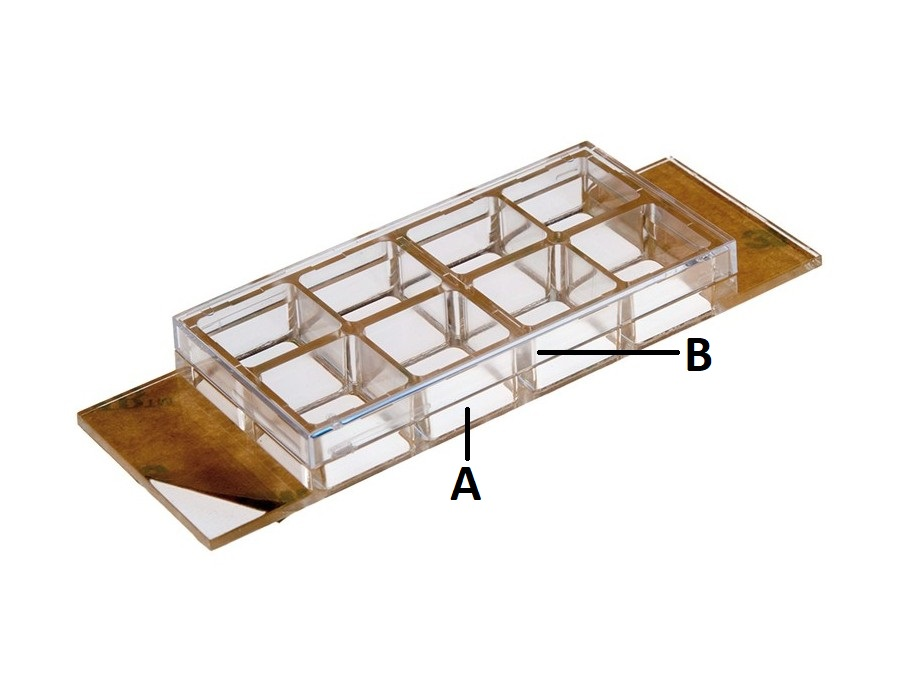
\includegraphics[width=0.6\textwidth]{images/sticky-slide-8-well-marked}
\caption{ibidi\textsuperscript{\textregistered} sticky-Slide 8 Well. The base SU-8 wafer is located in each of the containment box \textbf{(A)}. The SU-8 wafer is then fabricated in the surface of each containment box using nano photolitographic printing. The microfluidic system is then poured and stamped on top the wafer (see Appendix \ref{appendix:microtrench} for detailed manufacturing process). Note that each containment box is upside-open. The cap (\textbf{(B)} is used to prevent the ingress of foreign materials into the medium. \textit{Image taken and modified from ibidi GmbH's website}.}
\label{fig:ibidi}
\end{figure}

\begin{figure}[H]
\centering
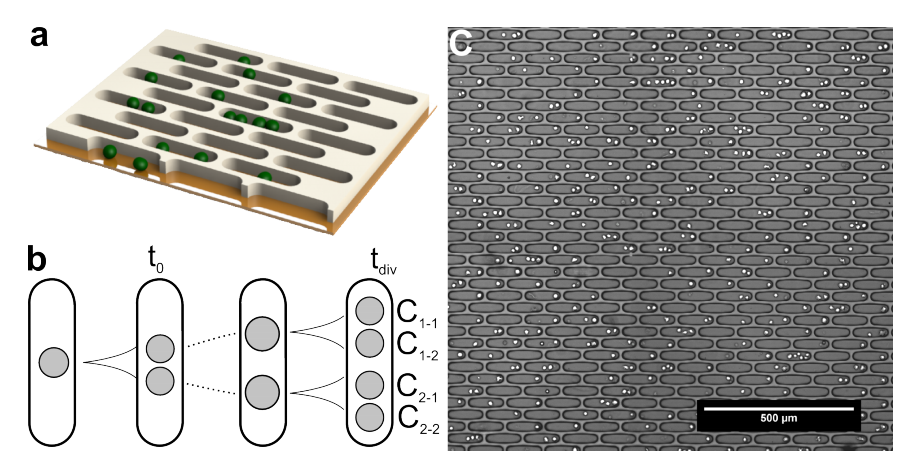
\includegraphics[width=1\textwidth]{images/trenches-sekhavati}
\caption{The structure of micro-trenches: \textbf{(A)} 3D model of micro-trench on surface with cells inside. \textbf{(B)} The schematic representation of a time-lapse in a trench. First, a singly-placed cell is tracked in a micro-trench. At time $t_0$, the cell divides into two daughter cells. The two cells will be kept tracked until at one point each of the daughter cells will divide at the same time at time $t_{div}$. Note the simplification of the sample. First, not every cell is singly-placed inside a trench. Indeed, not every trench is occupied by cells. Second, not every cell divides. Third, not every cell line observed has three generations in it. And finally, not every children's division times are at the same time. Indeed, this special case almost never happens in real life. \textbf{(C)} The sample view into the environment with cells occupying some micro-trenches. Here, the micro-trenches have dimension of 120 $\mu m$ long and 30 $\mu m$ wide. Note also the pointish characteristic of the cells taken in out-of-focus fashion. This improves the performance of the tracking algorithms. \textit{Figure taken from (Sekhavati, 2015) \cite{sekhavati2015dynamic}}.}
\label{fig:microtrench_design}
\end{figure}

\begin{figure}[H]
\centering
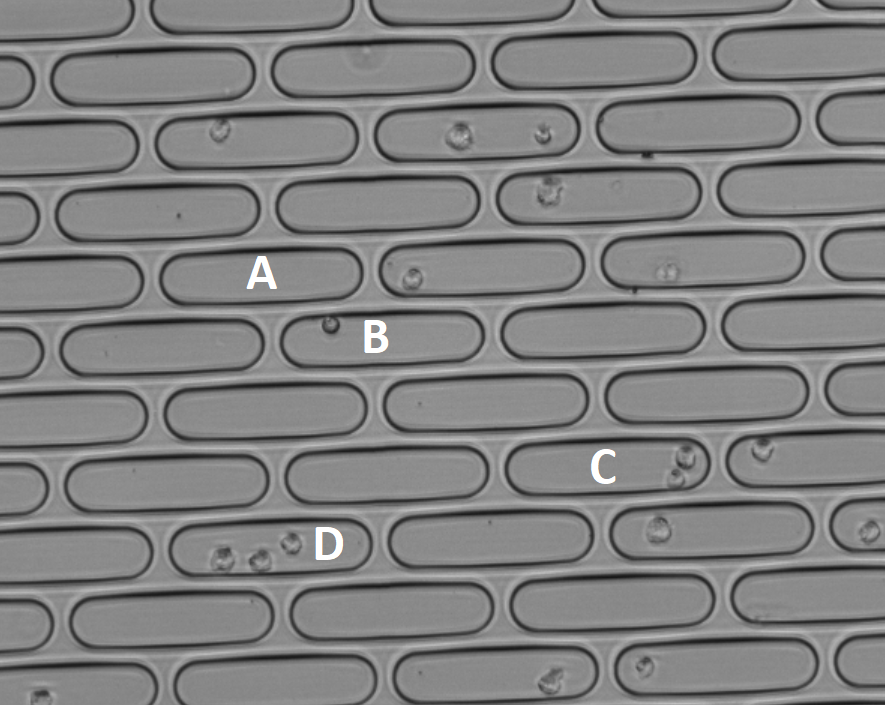
\includegraphics[width=0.8\textwidth]{images/microtrench_in}
\caption{The typical view of micro-trench setting. Some trenches contain no cell at all \textbf{(A)}. Several trenches contain exactly one cell \textbf{(B)}. A few more trenches contain two cells \textbf{(C)} while in rare cases the trench may contain more than two cells \textbf{(D)}.}
\label{fig:microtrench_sample}
\end{figure}

\subsection{Cancer Treatment Regimes}
\label{subsection:treatment}

As mentioned in previous chapters, the objective of the project partains mostly the dynamics of single cancer cell under treatment. After mentioning the cell lines of interest (Chapter \ref{subsection:cell_culture}) and the microfluidic setup used to contain cancer cells in single-cell setting (Chapter \ref{subsection:microfluid_env}), we arrived at the last aspect of the experimental seting: the chemical treatment used on the cells.

For cell cultures mentioned in chapter Subsection \ref{subsection:cell_culture}, two treatment regimes are developed : Vincristine and Daunorubicin -- both chemotherapeutic compounds well known for treating various kinds of cancer \cite{drugs2018defdaunorubicin, ravina2011evolution, tsuruo1981overcoming, gewirtz1999critical}.

\subsubsection*{Vincristine}

Vincristine is initially isolated from Madagascar pairwinkle \textit{Catharanthus roseus} (basionym \textit{Vinca roseus}, hence the name) \cite{nci2018defvincristine}. It is mainly known as Tubulin polymerase inhibitor \cite{tsuruo1982increased}, a subclass of mitotic inhibitor family of drugs \cite{jordan1998tubulin}. Mechanistically, it prevent Tubulin polymerization in two ways. First, it binds elongating Tubulin polymer and reduces the affinity of the elongating polymer \cite{lobert1996interaction} towards the monomers that are supposed to conjoin the polymer thereby extending it. Meanwhile, further elongation by the polymers are also prevented via allosteric inhibition (inhibition caused by spatial occupancy of inhibiting agent) of polymerating Tubulin via Vincristine. The allosteric competitor is hence commonly known as vinca alkaloid binding domain and commonly seen in other tubulin polymerization inhibitor compounds \cite{tsuruo1982increased}. It has also been shown that Vincristine also depolymerizes stable microtubuli in rat axonal part of rats' neuronal cells \cite{jordan1998tubulin}. Thus, the effect of Vincristine is most emphasized during the time of high Tubulin synthesis: during the separation of chromosomes in Metaphase by means of tearing them with the simultaneous pulling and pushing mechanism of Tubulin poly- and depolymerization \cite{owellen1972binding}. In the context of chemotherapy, Vincristine is often as combination in CHOP (cyclophosphamide, doxorubicin, vincristine, and prednisone) regime \cite{hiddemann2005frontline} against non-Hodgkin's lymphoma; MOPP \cite{brandriff1994chromosomal}, COPP \cite{pfreundschuh1987lomustine} and BEACOPP \cite{diehl1998beacopp} regimes against Hodgkin's lymphoma; and Stanford V regimes against acute lymphoblastic leukimia \cite{bartlett1995brief}. It is also used to certain degree as immunosuppresant due to its mitotic inhibiting characteristics \cite{ahn1974vincristine}.

\begin{figure}[H]
\centering
\begin{subfigure}{.8\textwidth}
  \centering
  
\includegraphics[width=.6\textwidth]{images/vincristine}
  \caption{}
  \label{fig:vincristine}
\end{subfigure}
\centering
\begin{subfigure}{.9\textwidth}
  \centering
  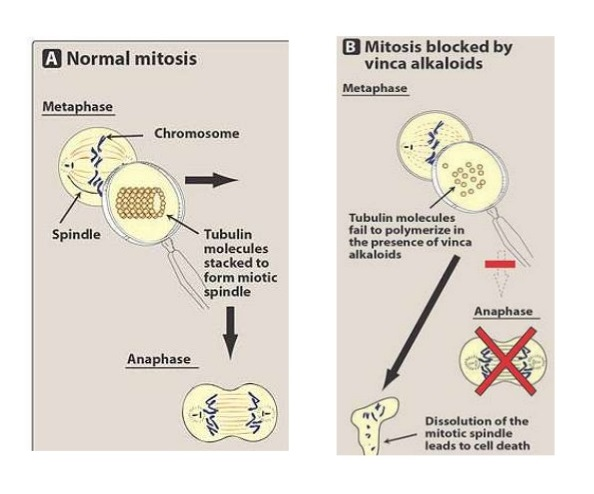
\includegraphics[width=.8\textwidth]{images/vincristine_mechanism}
  \caption{}
  \label{fig:anthracyclines_dna}
\end{subfigure}
\caption{(a) Molecular structure of Vincristine. (b) Visualization of Vincristine's mechanism of action. During normal metaphase, microtubuli elongate from centrosome towards equator and bind fully replicated chromosomes. The microtubuli then pull chromosome pair apart during anaphase. Vincristine and other vinca alkaloids prevent this from happening by competitive inhibition, allosteric inhibition and active depolymerization of extending microtubuli. Unsuccessful exit metaphase forces the cell to undergo programmed cell death.}
\label{fig:vincs}
\end{figure}

\subsubsection*{Daunorubicin}

Daunorubicin is initially isolated from bacterium \textit{Streptomyces peucetius} \cite{otten1990cloning, lin2011chiral}. It is part of anthracycline class of drug \cite{gewirtz1999critical} extracted mainly from \textit{Streptomyces} bacteria. Some well-known members of this class are Doxorubicin \cite{nci2018defdoxorubicin}, Epirubicin \cite{nci2018defepirubicin} and Idarubicin \cite{nci2018defidarubicin}. Together, they are among the most effective cancer drugs ever deployed and are used towards more kinds of cancer than other group of chemotherapeutic agents \cite{weiss1992anthracyclines, minotti2004anthracyclines, peng2005cardiotoxicology}. Like many chemotherapeutic agents including Vincristine, anthracyclines attack cancerous tissues and cells by preventing their division \cite{drugs2018defdaunorubicin}. Unlike vinca alkaloids however, anthracyclines prevent the division by disrupting another mechanistic part of cell division: the DNA polymerization \cite{gewirtz1999critical}. There are four ways anthracyclines disrupt DNA polymerization:

\begin{itemize}
\item Anthracyclines intercallate with base pairs involved in polymerization thus preventing strands extension \cite{takimoto2008principles}.

\item Anthracyclines covelatently inhibit of type II topoisomerase which is responsible for RNA and DNA supercoil relaxation \cite{wang2002cellular}. Inhibition of type II topoisomerase causes supercoiled RNA and DNA to be inaccessible for initiation of duplication thus breaking the DNA \cite{tewey1984adriamycin}.

\item Anthracyclines induce oxidative stress on cancer cell organelles by generating free oxygen radicals. These radicals in turn damage DNA, proteins and cell membranes and initiate caspase induced apoptosis \cite{vsimuunek2009anthracycline, halliwell1994free}.

\item Anthracyclines disrupt epigenetic, transcriptomic and DNA upstream regulations by removing histones from DNA strands \cite{pang2013drug}. This also exposes DNA strands to degradation factor such as DNA methylase \cite{vaissiere2008epigenetic} and oxidative damage \cite{ljungman1992efficient}

\item In presence of formaldehyde, anthracyclines cross-links with DNA covalently, creating cytotoxin that will disrupt DNA from functioning properly \cite{wang1991formaldehyde}.
\end{itemize}

In normal chemotherapeutic regime, both Vincristine and Daunorubicin are prescribed intravenously to the patients \cite{skeel2011handbook}. Needless to say, both drugs will disrupt both cancerous and healthy cells. The effect is however mostly felt in actively dividing cells and organs such as blood cells  and hair follicles due to chemotherapeutic agents' mostly disruptive effect during cell division as mentioned above \cite{skeel2011handbook, mayo2018chemotherapy}.

\begin{figure}[H]
\centering
\begin{subfigure}{.8\textwidth}
  \centering
  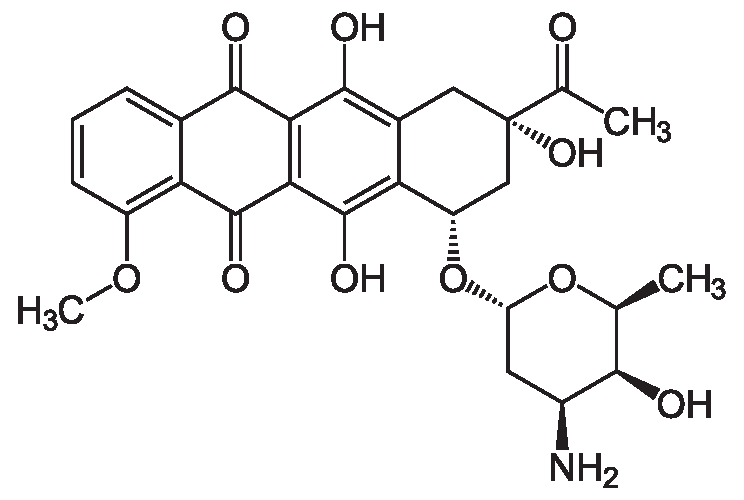
\includegraphics[width=.5\textwidth]{images/daunorubicin}
  \caption{}
  \label{fig:dauno}
\end{subfigure}
\centering
\begin{subfigure}{.8\textwidth}
  \centering
  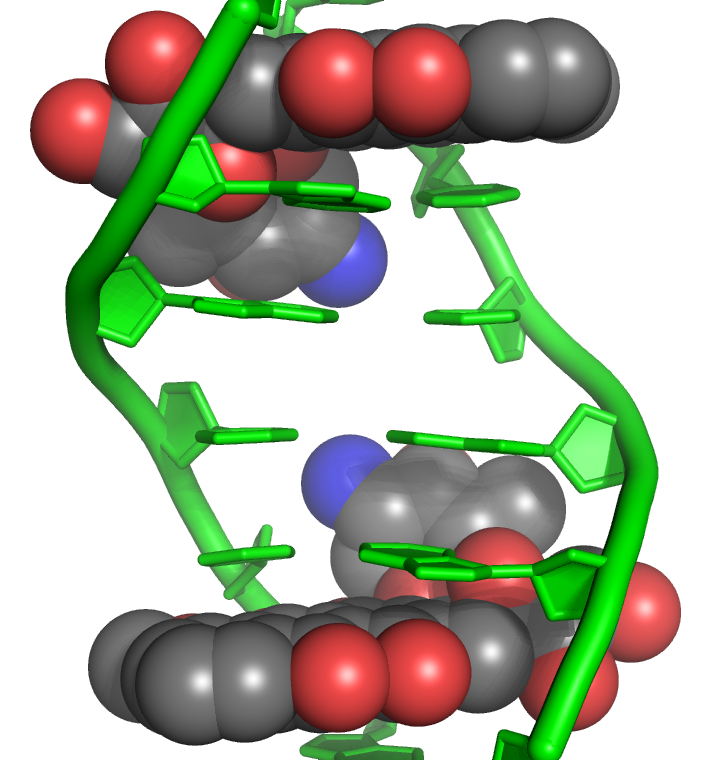
\includegraphics[width=.5\textwidth]{images/doxorubicin_dna}
  \caption{}
  \label{fig:anthracyclines_dna}
\end{subfigure}
\centering
\begin{subfigure}{.9\textwidth}
  \centering
  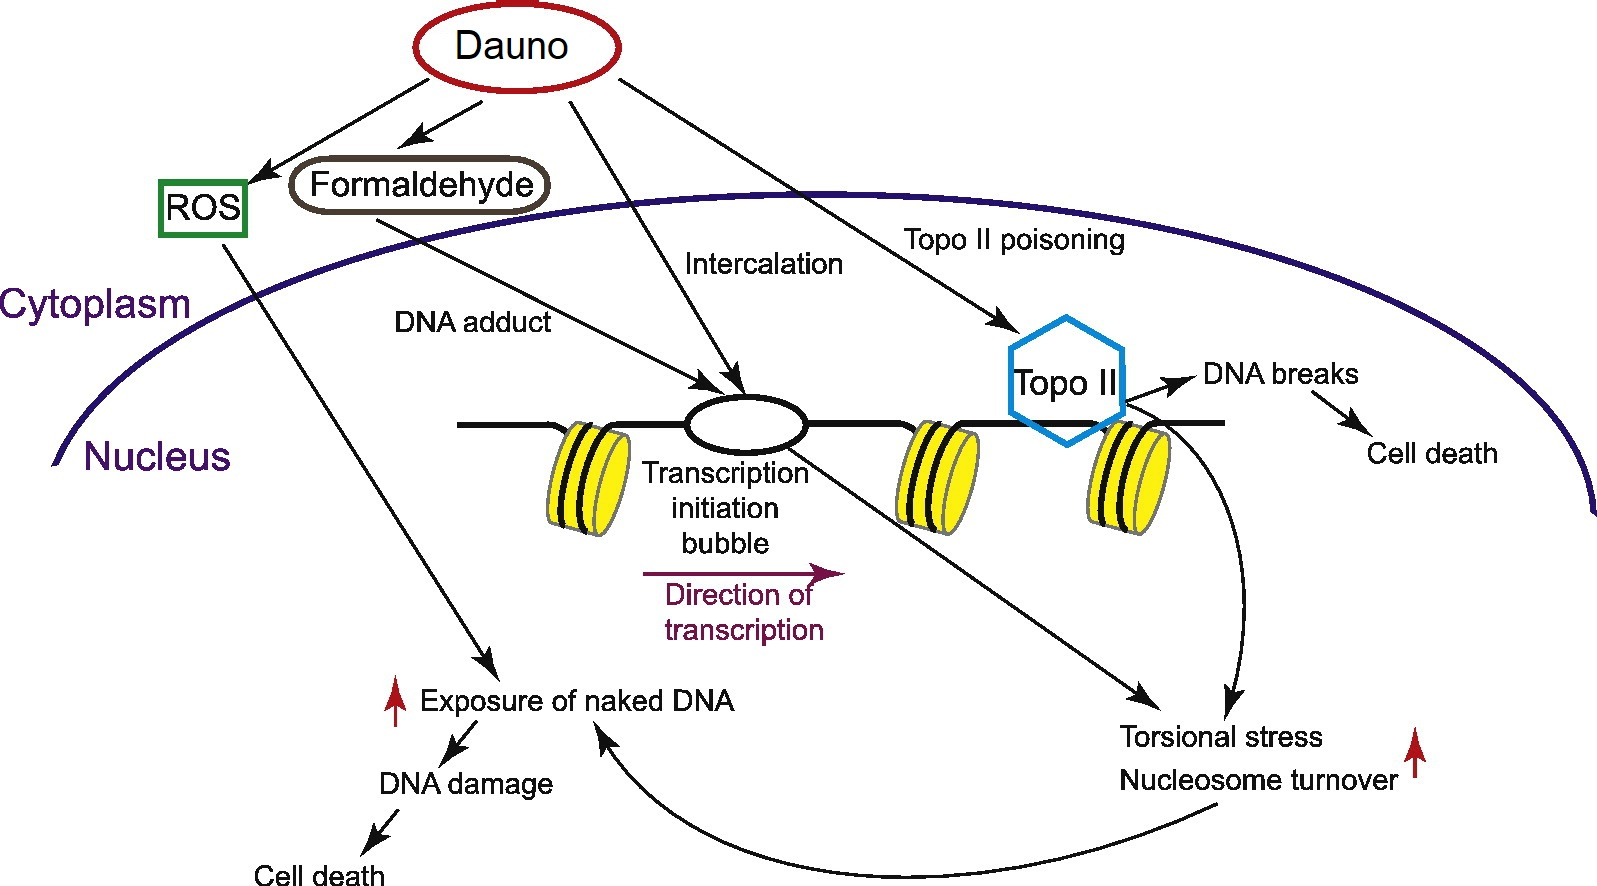
\includegraphics[width=.8\textwidth]{images/daunorubicin_mechanism}
  \caption{}
  \label{fig:dauno_mechanism}
\end{subfigure}
\caption{(a) Molecular structure of Daunorubicin. (b) Two anthracyclines intercalating with DNA double helix. (c) Schematic diagram of Daunorubicin's mechanism of action. From left to right: daunorubicin induce reactive oxygen species (ROS) which damage the DNA. Daunorubicin interfers with DNA by (1) covalently crosslinking with DNA mediated by formaldehyde and (2) intercalating DNA double helix. Daunorubicin also inhibits Topoisomerase II which prevents DNA supercoil's relaxation. Not shown in image: daunorubicin removes histone (shown in yellow in image) which disrupt epigenetic regulations. Modified from (Yang et al, 2014 \cite{yang2014doxorubicin}).}
\label{fig:daunos}
\end{figure}

\subsection{Cell Death Signal}
\label{subsection:cell_death_signal}

As mentioned in Subsection \ref{subsection:treatment}, the introduction of cancer treatment disrupts mitotic cell activities which in turn activates cell death pathways. To 

%TODO expand

\subsubsection*{Caspase 3/7}

%TODO expand

\subsubsection*{Propium Iodide (PI)}

%TODO expand

\subsection{Cell Treatments}
\label{subsection:cell_treatments}

Generally, following questions are to be investigated in the experiment:

\begin{itemize}
\item We would like to investigate the dynamics of the AML-M5a MOLM-13 cell line's response towards chemotherapeutic treatment regimes in various drugs' concentration levels (for both Vincristine and Daunorubicin).
\item We also would like to look into the effect of cell cycle on the the AML-M5a MOLM-13 cell line's response to drugs. Specifically, following questions needs to be answered: does the response of cancer cells depends on cell cycle?
\end{itemize}

To answer aforementioned questions, we designed the experiments as follow. First, two experiments are done:

\subsubsection*{Unsynchronized experiment.}

In the unsynchronized experiment, all 8 wells of the ibidi\textsuperscript{\textregistered} sticky-Slide 8 Well ('slide') are used with one microtrench wafer in each well (see Subsection \ref{subsection:microfluid_env} for the description of the slide). Wvery well is poured with different concentrations of treatments. To cover as many concentration range as possible, logarithmic scale is used to select concentration starting with 1 nanomolar (nM) all the way to 1000 nM. The use of logarithmic scale is also in line with logarithmic nature of many enzymatic and molecular process in cell biology \cite{wilkinson1961statistical, savageau1969biochemical}. Following concentrations are used:  1 nM, 5 nM, 10 nM, 100 nM and 1000 nM of Vincristine; 10 nM and 100 nM of Daunorubicin; and control concentration (0 nM). The unsynchronized experiment concentration configuration can be seen in Table \ref{table:unsyn_treatments}. The recording lasts for 45 hours. After 21 hours of recording, the chemotherapeutic treatment is introduced into each well. Table \ref{table:image_capture_frequency} shows the image capturing frequency for each image type.

\begin{table}[H]
\centering
\begin{tabular}{| l | c |}
\hline
Condition & Positions \\
\hline
A1: 1000 nM - VCR & 1-8 \\
A2: 100 nM - VCR & 9-15 \\
A3: 10 nM - VCR & 16-23 \\
A4: 1 nM - VCR & 24-31 \\
B4: 10 nM - Dauno 32 & 32-39 \\
B3: 100 nM - Dauno & 40-47 \\
B2: 0 nM - VCR & 48-55 \\
B1: 5 nM - VCR & 56-63 \\
\hline
\end{tabular}
\caption{Configuration table of treatments for synchronized experiment}
\label{table:unsyn_treatments}
\end{table}

\begin{table}[H]
\centering
\begin{tabular}{| l | l | c |}
\hline
What & What for & $t$ \\
\hline
In-focus brightfield (BF) image & Sanity check, micro-trench masking & 30 minutes \\
Out-of-focus BF image & Image tracking, image analysis & 15 minutes \\
Red fluorescence channel (PI)& Image tracking, image analysis & 15 minutes \\
Green fluorescence channel (Csp3/7) & Image tracking, image analysis & 15 minutes \\
\hline
\end{tabular}
\caption{Image capture frequency of the unsynchronized experiment}
\label{table:image_capture_frequency}
\end{table}


\subsubsection*{Synchronized experiment}

The main difference between unsynchronized and synchronized experiments is, as the name already suggests, the synchronization step done in synchronized experiment. The process involves arresting cell cycle with the so-called "double thymidine block" protocol \cite{harper2005synchronization}, which arrests cell development at $G_1/S$-phase by stopping DNA synthesis using double thymidine block, a well known DNA synthesis inhibitor \cite{bostock1971evaluation}.

Like unsynchronized experiment, several concentration levels are tested in this experiment (see Table \ref{table:syn_treatments}). The image capturing starts after the cells are synchronized and lasts 24 hours. The image capturing frequency is exactly the same as unsynchronized experiment's (see Table \ref{table:image_capture_frequency}).

\begin{table}[H]
\centering
\begin{tabular}{| l | c |}
\hline
Condition & Positions \\
\hline
A1: 1000 nM - VCR & 1-8 \\
A2: 100 nM - VCR & 9-15 \\
A3: 10 nM - VCR & 16-23 \\
A4: 1 nM - VCR & 24-31 \\
B4: 0 nM & 32-39 \\
B3: 5 nM - VCR & 40-47 \\
B2: 10 nM - Dauno & 48-55 \\
B1: 100 nM - Dauno & 56-63 \\
\hline
\end{tabular}
\caption{Configuration table of treatments for synchronized experiment}
\label{table:syn_treatments}
\end{table}

The detailed image capturing protocol for both unsynchronized and synchronized experiments can be seen in Appendix \ref{appendix:imageacquisition}.

\section{Definitions}

This section contains formal definitions used in this thesis.

\subsection{Image Encoding}
\label{subsection:image_encoding}

From the initial recordings on, there are several image standards and encodings being processed and analyzed in our pipeline. We would start from the raw image captured by recording apparatus going down to processed images (See Appendix \ref{appendix:imageacquisition}	 for detailed protocols on image acquisition).

There are two kind of recordings taken in our project: brightfield channel and fluorescence channel recordings. Two brightfield channels are used in this experiment:

\begin{itemize}
\item In-focus brightfield image. The focal distance of the camera $d_f$ is exactly the same as the distance from the apparatus to the microfluidic system $d_m$, i.e. $d_f = d_m$.
\item Out-of-focus brightfield image. To capture out-of-focus brightfield image, $d_f$ should be different than $d_m$. Several distances were tried during the experiments (see Figure \ref{fig:focustest}). Difference in focus-microfludics distance influences the quality of the image in several ways (see Figure \ref{fig:focustest}). It was determined that the best resulting image came from the lense with $d_f - d_m = -20 mu m$.
\end{itemize}

\begin{figure}[H]
\centering
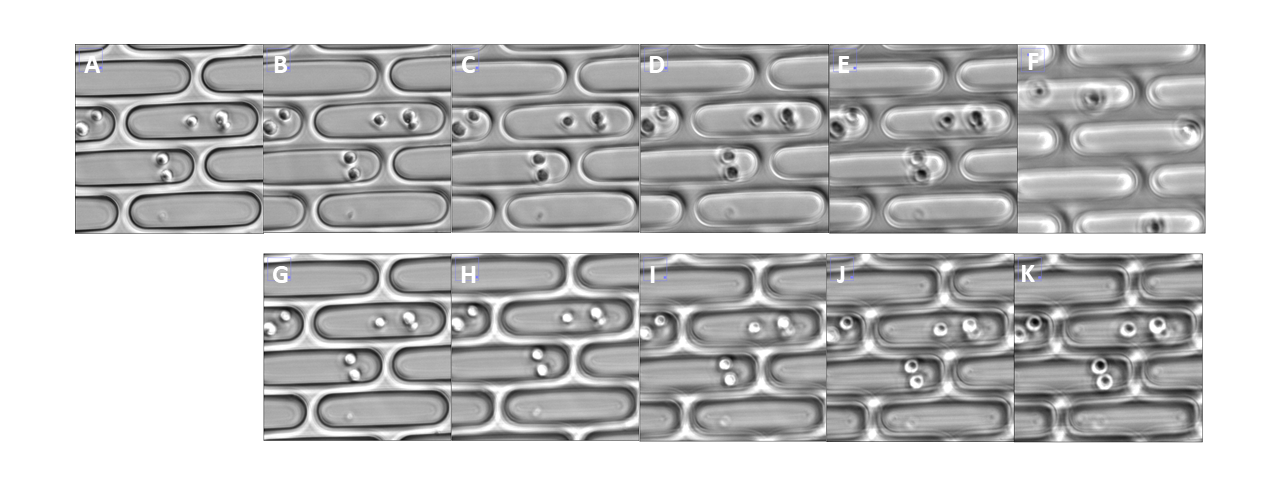
\includegraphics[width=\textwidth]{images/focus/pict.png}
\label{fig:focustest}
\caption{Comparison between in-focus image and out-of-focus images taken at various focus-microfluidics difference $d_f - d_m$. The images were taken from the section in the well. In the first row are images with focus behind the microfluidics system while in the second row are images with focus before the system. A: in focus image. B: $+10 \mu m$. C: $+20 \mu m$. D: $+30 \mu m$. E: $+40 \mu m$. F: $+50 \mu m$. G: $-10 \mu m$. H: $-20 \mu m$. I: $-30 \mu m$. J: $-40 \mu m$. K: $-50 \mu m$.}
\end{figure}

To detect cell death signal, fluorescent channels are used: red and green. These channels only capture fluorescence emission in corresponding spectrum area (i.e. 620–750 $nm$ and 495–570 $nm$ respectively):

\begin{itemize}
\item Red fluoroscent channel. This channel is used to capture emission coming out of PI activation due to PI's DNA binding emission being mostly in red wavelength (see Subsection \ref{subsection:cell_treatments}).
\item Green fluoroscent channel. This channel is used to capture emission coming out of caspase3/7 activation due to caspase3/7's binding emission being mostly in green wavelength (see Subsection \ref{subsection:cell_treatments}).
\end{itemize}

From the recording apparatus, the image came as TIFF image (see Appendix \ref{appendix:imageacquisition} for the detailed protocols) \cite{loc2006tiff}. Each recorded stack consists of slices which. One slice represent a single image capture at a time point. Each stack is encoded using RGB color model. This includes fluorescent image in which each slice shows the intensity in corresponding color channel (red, green or blue) as monochromatic RGB image. 

RGB color model represents the pixel as a combination of red, green and blue color. This encoding is able to represent various spectra of human visible color and useful enough for most use cases \cite{sonka2014image, jayant1993signal}. The most commonly used RGB encoding is the 8 bit encoding. Here, each pixel is represented as an RGB pixel having red, green and blue color values ranging from 0 to 255. Mathematically, this means that each pixel $M_{t,x,y}$ of a slice captured at time $t$ in this image can be represented a triple, i.e.:

\begin{equation}
\label{equation:rgb_pixel_def}
M_{t, x, y} := (M_{t, x, y, 1}, M_{t, x, y, 2}, M_{t, x, y, 3})
\end{equation}

with

$$
M_{t, x, y, 1} M_{t, x, y, 2} M_{t, x, y, 3} \in [0,255]
$$

for 8-bit RGB encoding. Consequently, a slice $M_t$ of width $w$ and height $h$ is a 3-dimensional matrix of dimension $h \times w \times h$, i.e.

$$
M_i \in p_c^{w \times h \times 3}
$$ 

with $p_c \in [0:255]$. A stack (a sequence of slices) $M$ of $n$ slices is in turn a 4-dimensional matrix:

$$
M_i \in p_c^{n \times w \times h \times 3}
$$ 

In some steps in the analysis pipeline, the image will modified to other encoding and vice versa, e.g. from 8 bit to 16 and from 8 bit to 32 bit RGB encoding. To convert RGB value of a pixel $M^a_{x,y}$ from one encoding to another $M^n_{x,y}$, linear conversion is normally used:

\begin{equation}
\label{euqation:linear_conv_rgb}
M^b_{x,y} = (\lceil M^a_{x,y, 1} \frac{2^b}{2^a} \rceil, \lceil M^a_{x,y, 2} \frac{2^b}{2^a} \rceil, \lceil M^a_{x,y, 3} \frac{2^b}{2^a} \rceil)
\end{equation}

where $a$ and $b$ refer to the bit length of the source and target encoding respectively (commonly known as \textbf{bid depth}).  Commonly used depths are 8, 16 (\textit{high color} format), 24 (\textit{true color} format) and 48 bits (\textit{deep color} format) \cite{lim1990two, sharma1997digital, sullivan2012overview}. 

Sometimes, both grayscale and 1-bit monochrome encoding is used/produced during image analysis. A grayscale image essentially shows the intensity of an image. A grayscale slice $G$ can be represented as matrix of integer, i.e. $G \in p_c^{w \times h}$ for 8-bit grayscale for example. Like RGB image, linear scaling can be applied to transform grayscale images across bit depth:

\begin{equation}
\label{equation:linear_conv_gray}
G^b_{x,y} = \lceil G^a_{x,y} \frac{2^b}{2^a} \rceil
\end{equation}

RGB image can be transformed to grayscale image by combining the intensity from every channel:

$$
G_{x, y} = \frac{M_{x, y, 1} + M_{x, y, 2} + M_{x, y, 3}}{3}
$$

this however does not reflect human perception of light, as human eyes' spectral sensitivity is not uniform across sensitivity spectrum \cite{wyszecki1982color}. Indeed, as Osorio and Vorobyev shows in 2005, each species has its own specific spectral sensitivity distribution \cite{osoosorio2005photoreceptor}, as can be seen in following figure:

\begin{figure}[H]
\centering
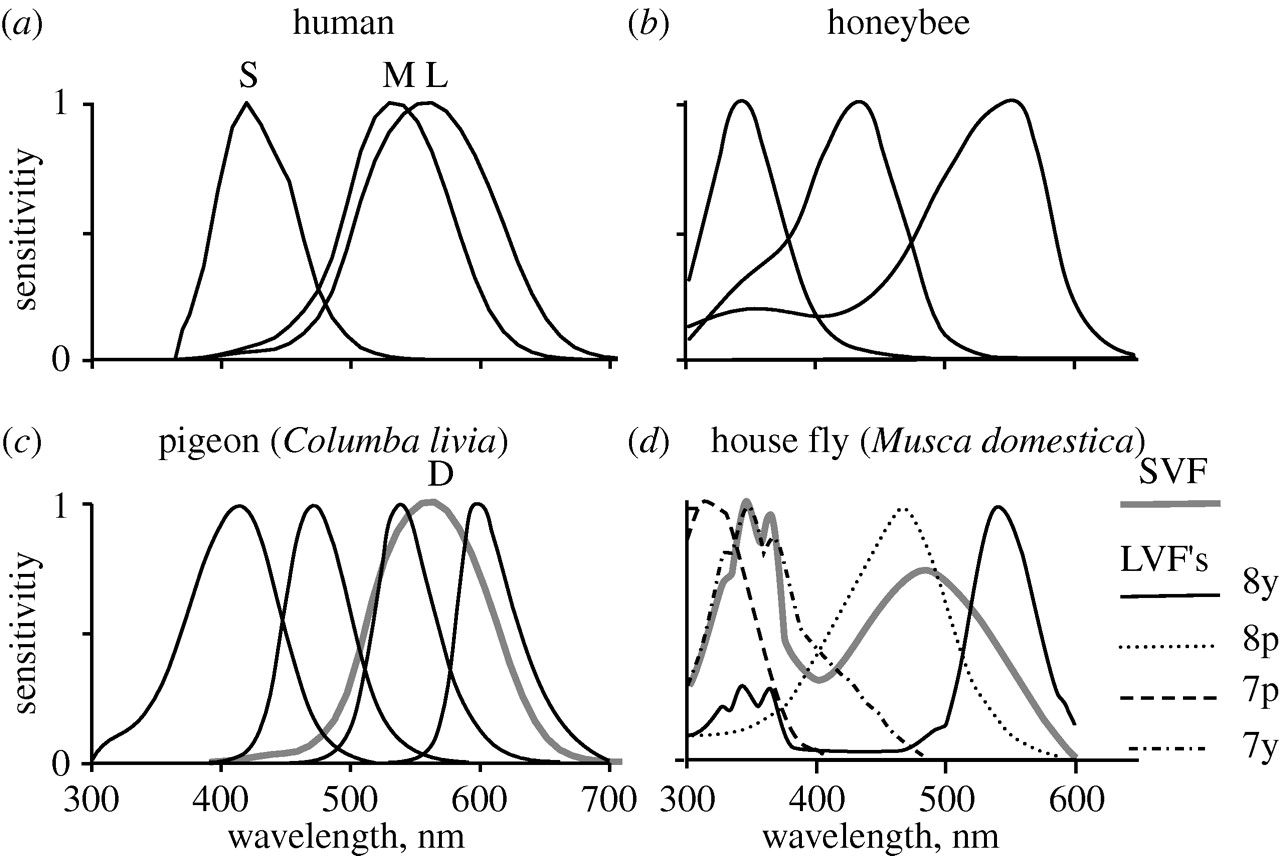
\includegraphics[width=0.5\textwidth]{images/spectral_sensitivity}
\label{fig:spectral_sensitivity}
\caption{Spectral sensitivity of human (a), honeybee (b), pigeon (c) and home fly (d). Note that the sensitivity distribution is maximum normalized (i.e. each value in a curve is relative only to the maximum value of the curve). Each species has its own set of cone cells, as can be seen in the variation of the number of curves for each species. D refers to double cone, while SVF refers to short visual fiber and LVF to long visual fiber. The y's and p's indicate the yellow/pale sensitivity of house fly's long visual fiber. Figure taken from (Osorio and Vorbyev, 2005 \cite{osorio2005photoreceptor}).}
\end{figure}

There are some conversions published on transforming RGB value to human intensity perception based on the measured spectral sensitivity \cite{anderson1996proposal, itu2007studio, itu2015parameter}. Among the most commonly used is the \textit{BT.601} standard from International Telecommunication Union (ITU). It recommends following luminosity weight for RGB to grayscale conversion \cite{itu2007studio}:

\begin{equation}
\label{equation:rgb_to_gray_def}
G_{x, y} = \frac{0.299 M_{x, y, 1} + 0.587  M_{x, y, 2} + 0.114 M_{x, y, 3}}{3}
\end{equation}

Reverting back grayscale to RGB image in turn only consists of applying grascale value to each color component:

$$
M_{x, y} := [G_{x, y}, G_{x, y}, G_{x, y}]
$$

A 1-bit monochrome image is encoded as binary matrix:

$$
B \in p_b^{w \times h} \land p_b \in {0, 1}
$$

this encoding is superior to other encoding for uses cases that do not require complete information of the image but rather separation of interesting parts in the image, since since it requires less memory (1 bit per pixel vs 24 bits per pixel of normal RGB image) and enables bitwise operation native to CPU \cite{kernighan1988c}. 

Some use cases for this encoding are for example region of interest (ROI) bounding and contour and boundary visualization \cite{hartley2003multiple}.

The conversion from RGB to binary image can be done by defining cutoff value $c$, i.e.

\begin{gather*}
B_{x, y} =
\begin{cases}
  1 & \text{if } M_{x, y} > c\\    
  0 & \text{else}  
\end{cases}
\end{gather*}

Note that, unless otherwise mentioned, every bit encoding of an image refers to unsigned encoding. Thus, an $m$-bit encoding allows value ranging from $0$ to $2^m - 1$.


%TODO take important things and remove
Consider the image of Lenna (Figure \ref{fig:lennasample}).

\begin{figure}[H]
\centering
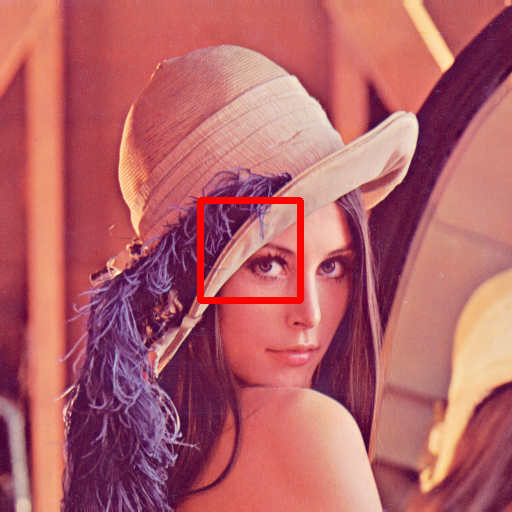
\includegraphics[width=0.5\textwidth]{images/lenna_marked}
\label{fig:lennasample}
\caption{Lenna}
\end{figure}

There are numerous encodings that could be used to internally represent this image. Many such encodings derived from the so-called Red-Green-Blue (RGB) encodings \cite{sonka2014image}. RGB encoding represents the pixel as a combination of red, green and blue color. This encoding is able to represent various spectra of human visible color and useful enough for most use cases \cite{sonka2014image, jayant1993signal}. To give representation on how the encoding works, the RGB encoding of some part of Figure \ref{fig:lennasample} is shown in Figure \ref{fig:lennas}. For an image of size $m \times n$ pixels, the RGB encoding is thus a 3-dimensional matrix of dimension $m \times n \times 3$. For time-lapsed images accordingly, the RGB encoding of a video of length $T$ is a 5-dimensional matrix of shape $T \times m \times n \times 3$. %TODO put graphical explanation of data here.

%An expansion of such encoding, the RGBH encoding, expands the representation by adding the brightness of the pixel -- known as 'hue'.

\begin{figure}[H]
\begin{subfigure}{.5\textwidth}
  \centering
  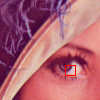
\includegraphics[width=.8\linewidth]{images/lenna_marked_small}
  \caption{}
  \label{fig:lennas1}
\end{subfigure}%
\begin{subfigure}{.5\textwidth}
  \centering
  
\includegraphics[width=.8\linewidth]{images/lenna_small}
  \caption{}
  \label{fig:lennas2}
\end{subfigure}
\centering
\begin{subfigure}{.5\textwidth}
  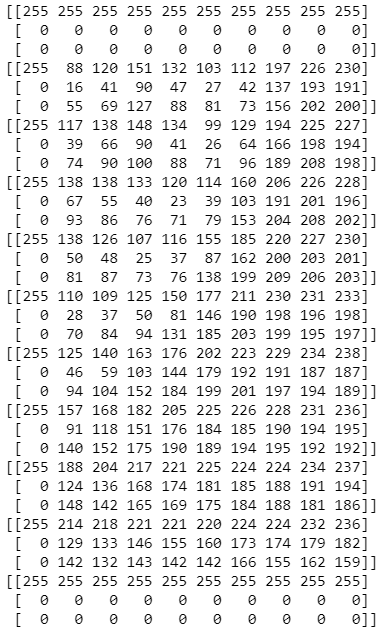
\includegraphics[width=.8\linewidth]{images/lenna_rbg}
  \caption{}
  \label{fig:lennas3}
\end{subfigure}
\caption{Figure \ref{fig:lennas1} shows the content of red marked region in Figure \ref{fig:lena}. Figure\ref{fig:lennas2} shows the zoomed part around Lena's right eye and matrix represented in Figure \ref{fig:lennas3} shows the RGB representation of the eye.}
\label{fig:lennas}
\end{figure}

\section{Methods}

\subsection{Brightness and Contrast adjustment}

We consider following image: 

\begin{figure}[H]
\centering

\includegraphics[width=0.4\textwidth]{images/pos_41_in_t0}
\label{fig:pos41}
\caption{The in-focus image of position 41 from unsynchronized experiment.}
\end{figure}

using RGB to intensity conversion formula shown in Subsection \ref{subsection:image_encoding}, we can convert the image into grayscale image representing the intensity. The grayscale image has the intensity distribution as shown in following histogram:

\begin{figure}[H]
\centering
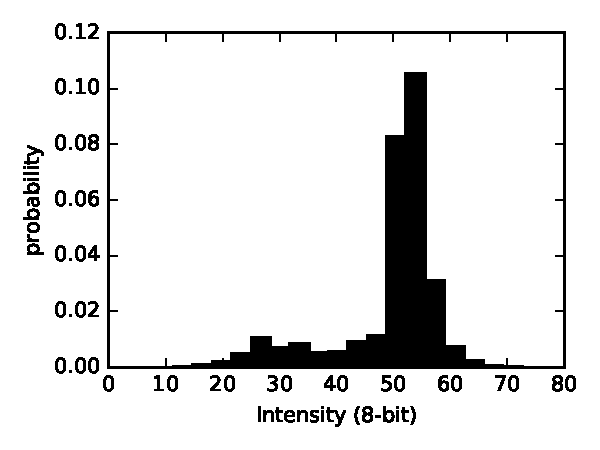
\includegraphics[width=0.4\textwidth]{images/pos_41_in_t0_hist}
\label{fig:pos41_density}
\caption{Normalized distribution of intensity of Figure \ref{fig:pos41}.}
\end{figure}

Mathematically, we can represent brightness and contrast adjustment as a mapping between one domain to another one. Let $l(M_{t, i, j})$ a function that maps the RGB value of a pixel $M_{t, i, j}$ to its corresponding intensity. Conventiently, we can use ITU's \textit{BT.601} standard the formula written in Subsection \ref{subsection:image_encoding}.

We then define the $I: [0:w] \times [0:h] \rightarrow \mathbb{N}_0$ function that maps the coordinate of a pixel to its corresponding intensity value i.e.

$$
I_t(i, j) := l(M_{t, i, j})
$$

Note that the codomain of the function $I_t$ depends on the encoding used. For a 8-bit encoding this will be then $[0:255]$.

An intensity transformation $J_t$ is then defined as a linear transformation of $I_t$ with \textbf{gain} and \textbf{bias} parameters $\alpha$ and $\beta$ respectively,

\begin{equation}
\label{equation:br_ct_transform}
J_t(i, j) := \alpha \cdot I_t(i, j) + \beta
\end{equation}

with $\alpha > 0$ \cite{szeliski2010computer}. The gain and bias parameters are also known as \textbf{contrast} and \textbf{brightness} parameters accordingly. In this regard, increasing/decreasing brightness is equivalent to increasing/decreasing $\beta$. The same thing also applies for contrast parameter, increasing $\beta$ will increase the brightness of the image.

Predictably, doing transformation over by $J_t$ will inevitably cause the resulting intensity to be outside of the allowed value range $[0:2^m]$ for m-bit encoding. To understand this situation, we first have to consider the boundedness of eyes perception. The argumentation for boundedness can be shown by realizing that the excitation of a neuron follows sigmoid function \cite{gazzaniga2004cognitive}. Thus given no impuls the neuron will stay in ground state, while very large impulse is bounded due to biochemical constraint of a neuron. Mapped in the context of sigmoid function, a steady state corresponds to 0 while asymptotically unlimited excitation correspondes to 1. In our context, a non-excited state corresponds to 0 intensity while full-excitation corresponds to $2^m - 1$ intensity. Thus, the equation \ref{equation:br_ct_transform} could be closely bounded by introducing upper and lower bound of $0$ and $2^m - 1$, i.e.:

\begin{gather*}
J_t(i, j) :=
\begin{cases}
  2^m - 1 & \text{if } \alpha \cdot I_t(i, j) + \beta > 2^m - 1\\
  0 & \text{if } \alpha \cdot I_t(i, j) + \beta < 0\\
  \alpha \cdot I_t(i, j) + \beta & \text{else}
\end{cases}
\end{gather*}

We can for example, transform Figure \ref{fig:pos41} using $J_t(i, j)$ with $\beta=100$. $\alpha$ is not changed in this case. Following images show the transformed image and its corresponding normalized intensity distribution:

\begin{figure}[H]
\centering

\begin{subfigure}{\textwidth}
  \centering
  
\includegraphics[width=0.4\textwidth]{images/pos_41_in_t0_br_up100}
  \caption{1a}
  \label{fig:pos41_brup100_bf}
\end{subfigure}%

\begin{subfigure}{\textwidth}
  \centering
  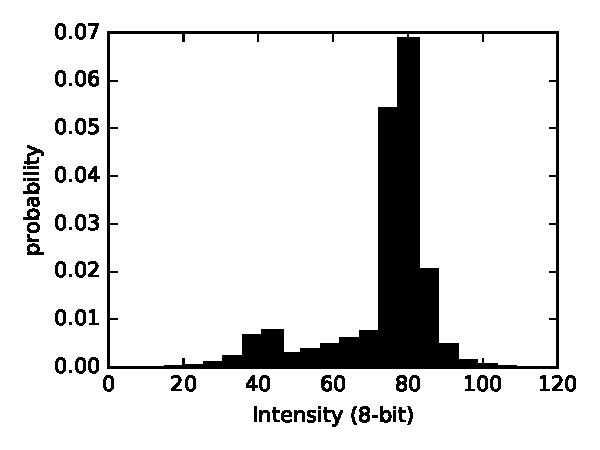
\includegraphics[width=0.4\textwidth]{images/pos_41_in_t0_br_up100_hist}
  \caption{}
  \label{fig:pos41_brup100_hist}
\end{subfigure}%

\label{fig:pos41_brup100}

\caption{(a) The in-focus image of position 41 from unsynchronized experiment tranoformed with $\alpha=1$ and $\beta = 100$. (b) Normalized distribution of intensity of the transformed figure.}
\end{figure}

We can also try to change $\beta$. This will scale the image's intensity and emphasize image contrast.

%TODO expand

\begin{figure}[H]
\centering

\begin{subfigure}{\textwidth}
  \centering
  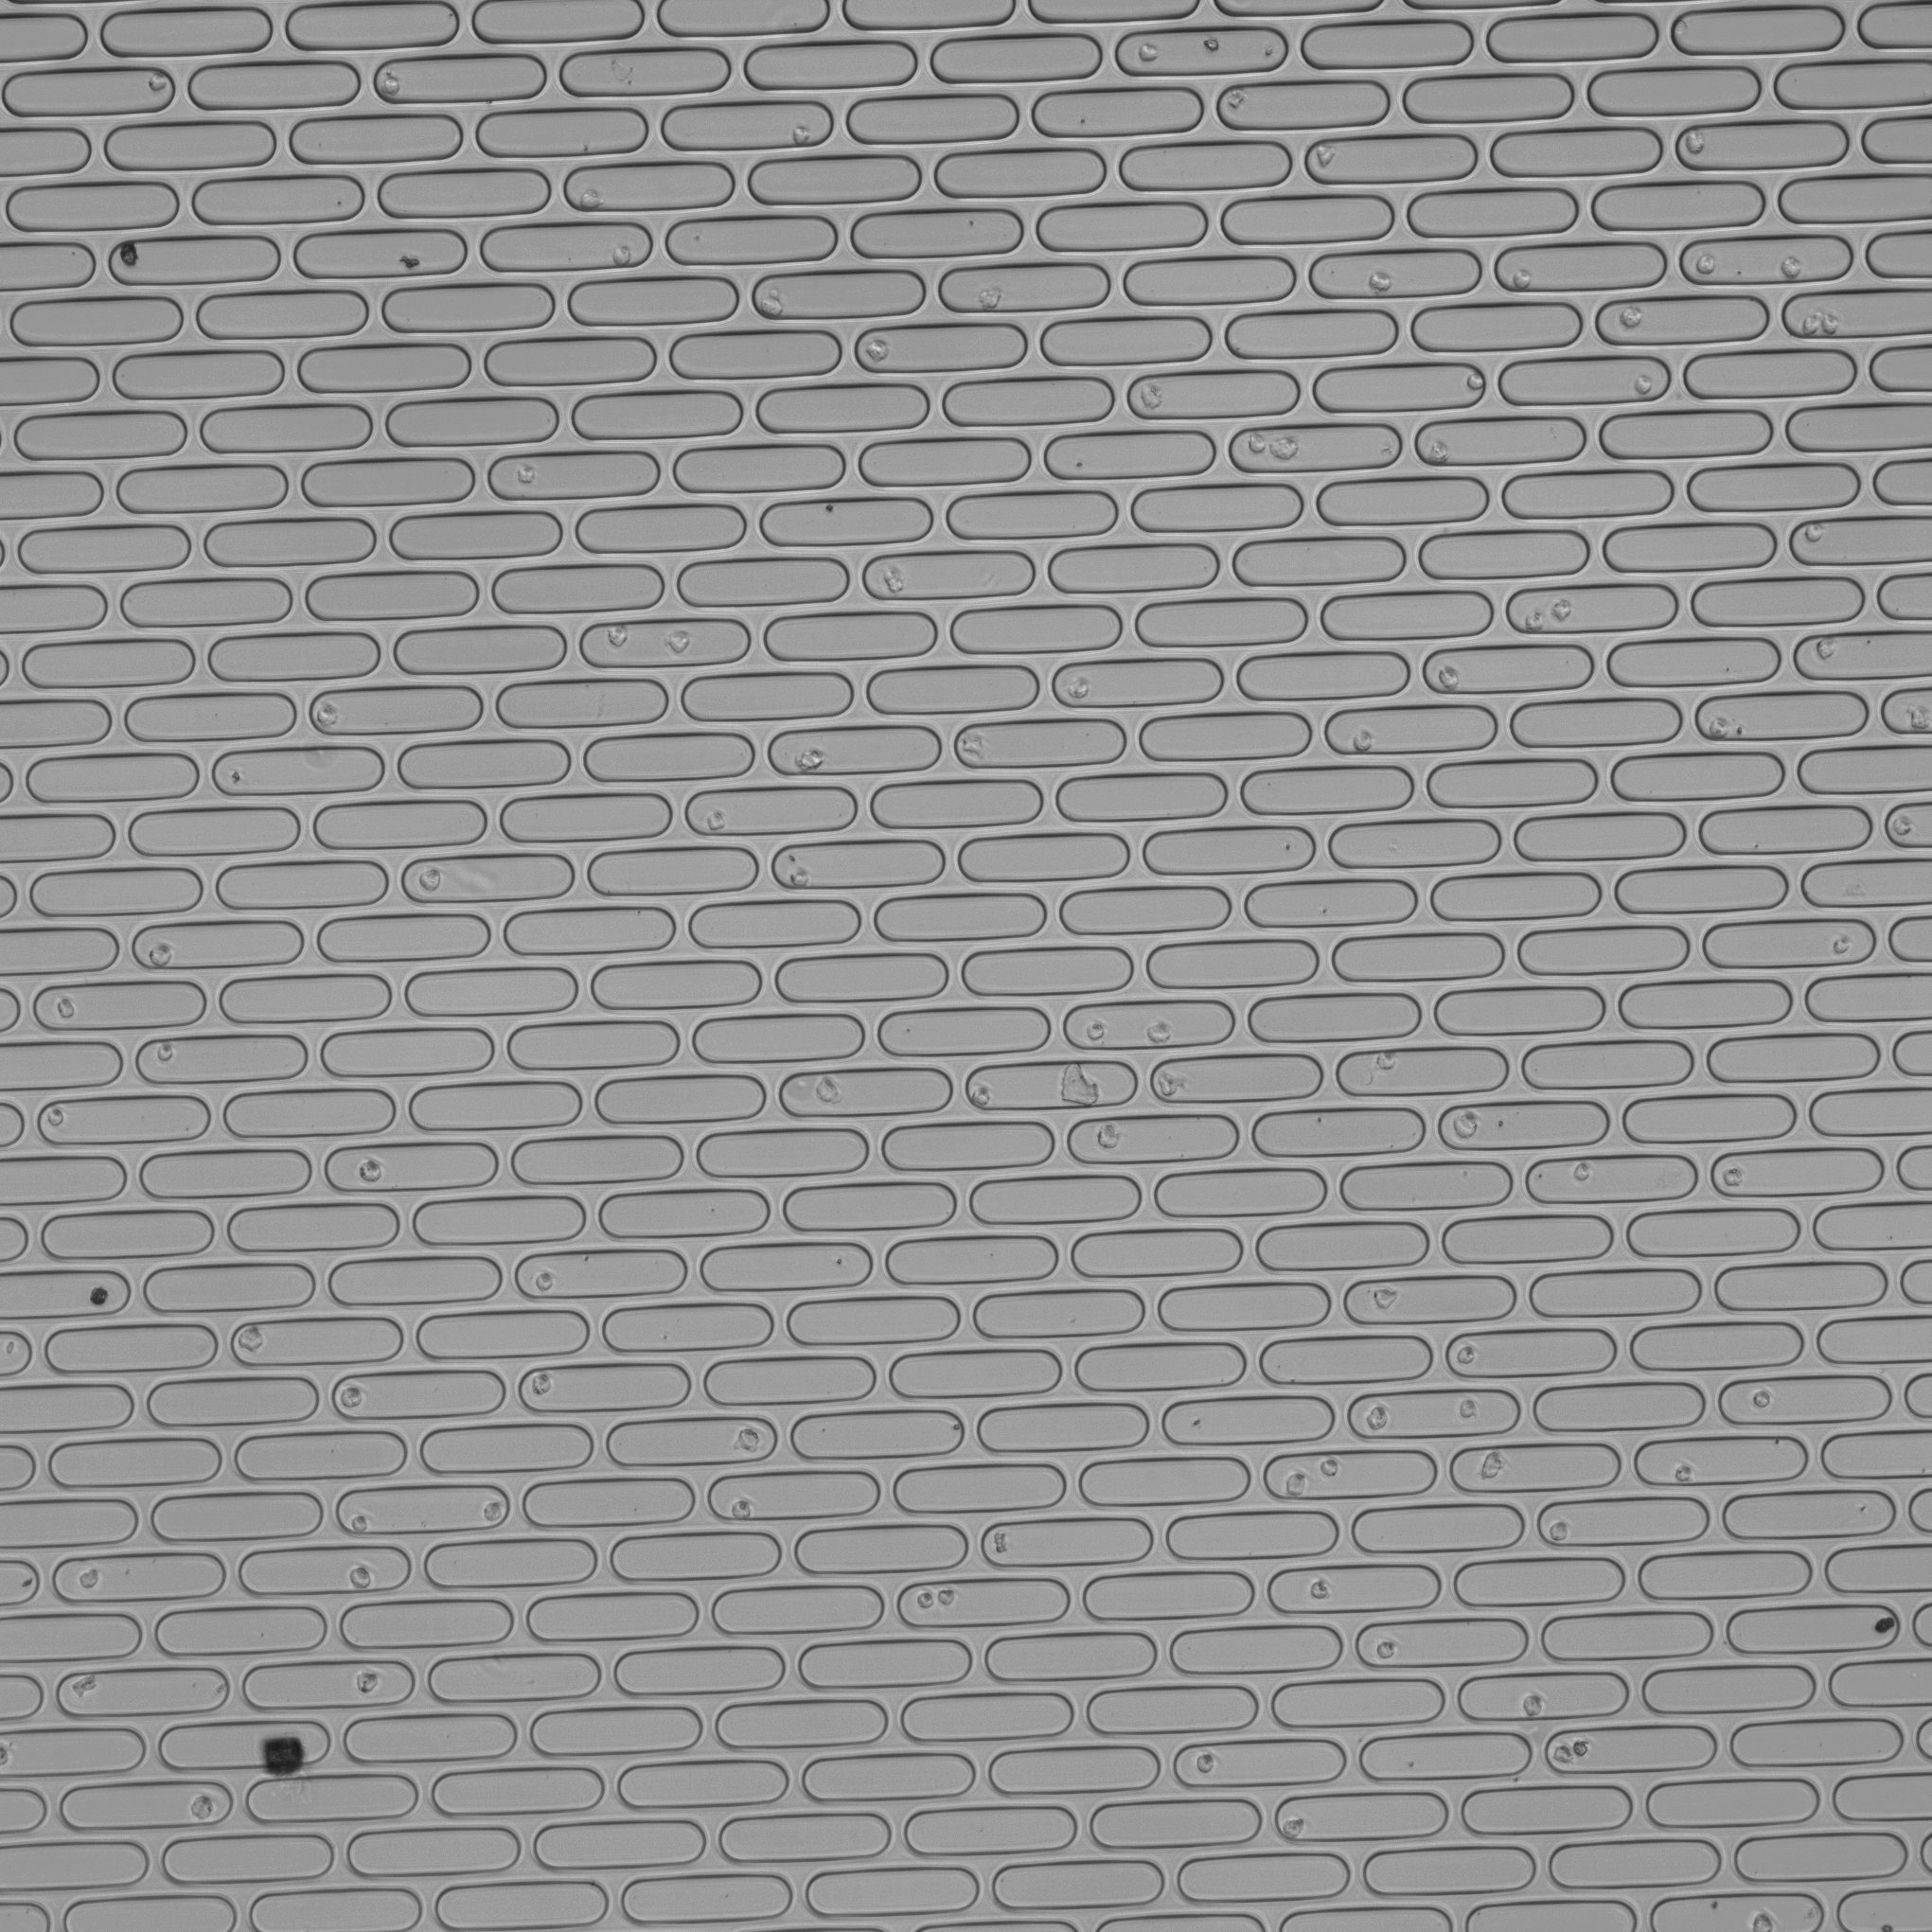
\includegraphics[width=0.4\textwidth]{images/pos_41_in_t0_br_times3}
  \caption{}
  \label{fig:pos41_times3_bf}
\end{subfigure}%

\begin{subfigure}{\textwidth}
  \centering
  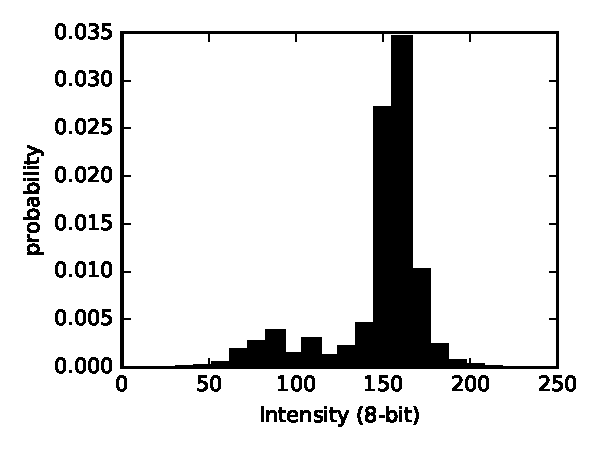
\includegraphics[width=0.4\textwidth]{images/pos_41_in_t0_br_times3_hist}
  \caption{}
  \label{fig:pos41_times3_hist}
\end{subfigure}%

\label{fig:pos41_times3}
\caption{(a) The in-focus image of position 41 from unsynchronized experiment tranoformed with $\alpha=3$ and $\beta = 0$. Notice the contrast has increased significantly, especially around area with high intensity differential such us the margin of a micro-trench and the dark spot in the lower left part of the slice. (b) Normalized distribution of intensity of the transformed figure}
\end{figure}

Geometrically, contrast can be understood as the distance of closely resembling pixel. Two pixels which are very similar will look very different given a high contrast. Brightness, on the other hands, describes the level of visibleness of a pixel.

\subsection{Slit Masking}

Several techniques could be applied to highlight certain area in the image (TODO citation, citation, citation). One  of such methods is detection using brightness composition \cite{cheng2015global}. We can see for example that the area around a micro-trench exposes the so-called strong intensity gradient: the area around the marging of a micro-trench is much darker than the other parts of the well. This can be explained by the fact that several. 

As mentioned in 
Consider the case in which 

\subsection{Gradient background correction}

Gaussian blurring

\subsection{Normalization of local contrast}

\subsection{Static correction}

\subsection{Cell Recognition}

Laplacian of Gaussian

\subsection{Cell Tracking}

Linear Assignment Problem

\subsection{Shift Correction}

Now, consider a case in which images are shifted in a time-lapsed movie. TODO: explain mechanism. No rotation of camera is assumed, hence there are only two degree of freedoms (vertical and horizontal). Thus, a shift can be defined as a vector movement $\vec{v}$ of all points $x_{i,j} \in M_{t_i}$ in the time-lapse from time $t_i$ to $t_{i+1}$. Given two degrees of freedom and discreteness of the problem due to pixel representation, the task is reduced to finding difference in x- and y-axis ($\delta_x$ and $\delta_y$), so that the difference of transformed pixels at $t_i$ and $t_{i+1}$ are minimized, i.e.:

$$
argmin_{\delta_x, \delta_y} \{d(M_{t_i}, M_{t_{i+1}}^{\delta_x, \delta_y} + (\delta_x, \delta_y)^T)\}
$$

Where $M_{t_{i+1}}^{\delta_x, \delta_y}$ is the entries of matrix $M_{t_{i+1}}$ after applying the shift $\vec{v} := (\delta_x, \delta_y)^T$, i.e.

$$M_{t_{i+1}, \, x, \, y}^{\delta_x, \delta_y} = M_{t_{i+1}, \, x - \delta_x, \, y - \delta_y}$$

For the distance function $d$, the in all channels absolute difference function is used, which is defined as:

$$
d(M_i, M_j) = \sum_{c \, \in \, \{R, B, G\}} \sum_{x} \sum_{y} \vert M_{i, c, x, y} - M_{j, c, x, y} \vert
$$


Since some pixels are lost from the field of view during a shift, only a subset of subsequent images is used to determine the shift, preferably those around the center point. This will allow the largest search space possible, since the distance to all four margins of the image is maximized at the center point. The search for the optimal $(\delta_x, \delta_y)$ pair is implemented as a grid search along the x- and y-axis. An example of the search grid is shown in Figure \ref{fig:searchgrid}.\\

\begin{figure}[H]
\centering
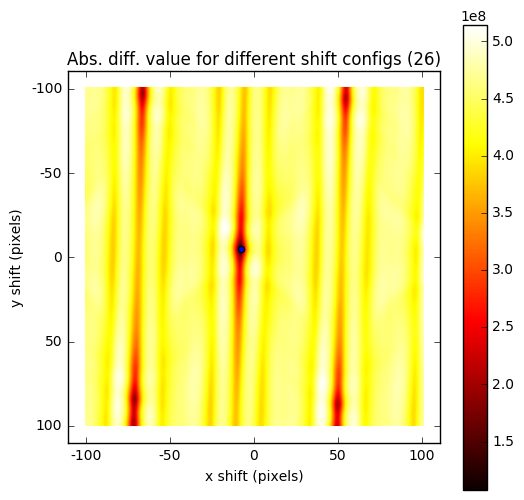
\includegraphics[width=0.5\textwidth]{images/search_grid}
\caption{Search grid shift for Position 26. The search was conducted for shift between the last time point before and the first time point after the drugs treatment. The minimum is marked with thick black dot, which is returned after every grid-search call as inferred shift. In the position, the shift was inferred to be 8 pixels upwards and 5 pixels leftwards. Notice the repeating pattern of relatively favorable configurations after approximately 50 horizontal and 100 vertical pixels caused by lattice nature of the trenches.}
\label{fig:searchgrid}
\end{figure}

%TODO : RESTRUCTURE THE CHAPTER

Since the time-lapsed data consists mainly of grayscale image, the RGB encoding could be the directly transformed to grayscale encoding. Using the transformed method also speeds up the calculation process since the distance function only computes the difference of grayscale channel's values:

$$
d(M, N) =  \sum_{x} \sum_{y} \vert M_{c, x, y}^{gray} - N_{x, y}^{gray}\vert
$$

Due to lost pixels around the margin of before and after images, only the overlapping part of both slides are included after the correction. Thus, for an inferred shift of $(\delta_x, \delta_y)$, the new dimension of the images is then $(m - \delta_x) \times (n - \delta_y)$. This change would then propagation to the other time-lapse images to maintain consistency of the images.\\

Ideally, the shift correction should be done for each position to reduce the track dropout rate caused by image shifts. This is however computationally very expensive and, as seen in Figure \ref{fig:pixdiff}, not really necessary since the biggest shift indeed only happens right before and after the treatment, as it was expected during the experiment setting. As seen in Chapter XX (TODO: quote), the tracking allows certain amount of tolerance. In this regard, the other frame shifts are way within the tolerance of our tracking algorithm. As shown in Figure YY (TODO: add droput rate), the dropouts caused by frame shifts in the other time points are basically noisy dropout caused by random noise in time-lapse movie being tracked as cells \cite{jaqaman2008robust}.

The algorithm for shift inference is available in Appendix \ref{appendix:algo}.

\begin{figure}[H]
\centering
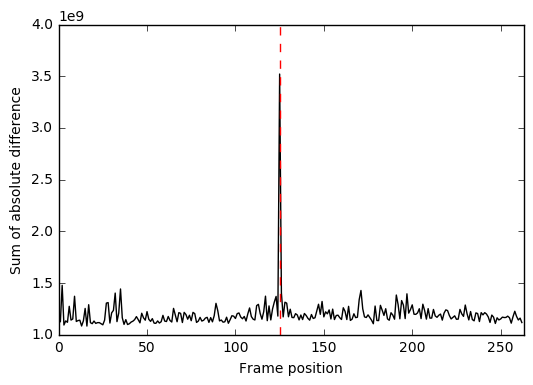
\includegraphics[width=0.8\textwidth]{images/pixdiff}
\caption{Pixel difference between consecutive frames at Position 26. In most cases, the pixel difference between the frames is mainly caused by moving cells. The diference during the treatment, on the other hand, is caused by physical shift of the frame. While moving cells mostly caused minimum noise-like pixel difference, the physical shift of field of view distorts the physical alignment and evokes immense pixel difference.}
\label{fig:pixdiff}
\end{figure}

\subsection{Cell death signals}

Measuring cell death is a crucial part of the experiment, as the reliable determination of it is the basis of most analysis in this thesis. There are several way to measure cell deaths with varying complexity and accuracy. Each method contains certain assumptions of cell death.\\

For example, determining cell death by cell movement assumes death of a cell if no movement beyond random flux is observed in certain amount of time. This obviously has certain drawbacks, such as when the observation is done in non-static environment. Moreover, defining the limit of the random flux, above which a given cell is assumed to actively move, is not a trivial task. Some kind of gold standard for a given cell line and environment has to be established manualy, which is very time consuming. This fact is again made even more complicated by the fact that many cells show different movement pattern upon introduction of treatment. It is well known that some cells tend to move faster or slower under stress, the situation many cancerous cells in our experiment will experience upon addition of cancer drugs treatment \cite{pienta1991effects, fenteany2003small, ruocco2012suppressing}.\\

The second method is using cell size. During apopotosis, the cells would shrink. Given It is known that cell size %TODO continue.

In this experiment, two cell signals are used as indicator of cell death. %TODO continue

\chapter{Analytic Pipeline}

\section{Pipeline Description}

\section{Pipeline Specification}

\chapter{Results}


\begin{verbatim}
I. Pipeline

II. Quantitative Analysis
\end{verbatim}

\section{Quantitative Analysis}

\section{Machine Learning Models}

\chapter{Summary and Outlook}

\section{Fully automated microfluidics pipeline}

\section{Fully automated image analysis pipeline}

\begin{verbatim}
I. Summary (and discussion?)
Connect Results with Background

II. Outlook
Improvemnt capability
\end{verbatim}

%% BIBLIOGRAPHY %%

\bibliographystyle{unsrt}
\bibliography{mabib}

%% APPENDICES %%

\begin{appendices}

\chapter{Experiment Protocols}

\section{Micro-trenches array fabrication} \label{appendix:microtrench}

\subsection*{Photolithography of the SU-8 wafer}

The fabrication of the SU-8 (MicroChem Corp, USA) wafer was executed in a in-house cleanroom facility using a ProtoLaser LDI system (LPKF Laser \& Electronika, Naklo, Slovenia), with a 375 nm wavelength laser and 1 μm spot diameter.

\subsection*{Softlithography and Micromolding}

Polydimethylsiloxane (PDMS) prepolymer solution is mixed with the crosslinker in a 10:1 ratio (w/w) (Sylgard 184, Dow Corning, USA) and then degassed under vacuum. PDMS is then purred on the SU-8 wafer, degassed and cured in 50 oC. The resulting PDMS stamp is peeled off the wafer and cut into appropriate shapes. The PDMS pieces, with 25 1/4 pillars in height, are activated with argon plasma and then immediately placed upside down on a silanized with TMSPMA (3-(Trimethoxysilyl)propyl methacrylate, Sigma-Aldrich) glass coverslip. A solution of PEG-DA (Mn=258) containing 2\% v/v of the 2-hydroxy-2methylpropiophenone (both from Sigma-Aldrich, Germany) is freshly prepared and then a drop is deposited at the edge of the PDMS stamp. The PDMS stamp is filled by capillary force induced flow. PEG-DA is then polymerized in an UV-ozone cleaning system (UVOH 150 LAB, FHR, Ottendorf, Germany). Next, the PDMS stamps are peeled off and the resulting micro-trenches of cross-linked PEG-DA are dried in an oven (Binder GmbH, Tuttlingen, Germany) overnight at 50oC. Finally, the slides are sonicated with 70\% ethanol and distilled water before a sticky slide is attached on top (8-well sticky slide, ibidi GmbH, Munich, Germany).

\section{Images Acquisition}
\label{appendix:imageacquisition}

Imaging was performed under an inverted Nikon Ti Eclipse microscope with a motorized stage (Tango XY Stage Controller, M\"arzh\"auser Wetzlar GmbH \& Co. KG, Germany), a CFI Plan Fluor DL 10X objective, a pco.edge 4.2 Camera (PCO AG, Kelheim, Germany) and a Lumencor Sprectra LED fluorescence lamp. For detection of the Caspase-3/7 and the PI marker, the following filters were used respectively, 474/27 nm, 554/23 (excitation) and 515/35 nm, 595/35 nm (emission). Brightfield out of focus (-20 $\mu$m) images were taken every 10 minutes and in-focus  brightfield and fluorescence images every 30 minutes for 48 hours. Vincristine or Daunorubicin were added after 20 hours from the beginning of the imaging. During the recording samples were kept at a constant temperature of 37\degree C and CO2 using an Okolab heating and CO\textsubscript{2} 2 box (OKOLAB S.R.L., NA, Italy). For the synchronized population, the double thymidine block protocol was followed. Briefly, MOLM-13s cells at the exponentially growing phase were incubated in blocking medium (culture medium supplemented with 2 mM Thymidine (CAS 50-89-5, Calbiochem\textsuperscript{\textregistered}, Germany)) for 24 hours. Cells were then released and incubated in culture medium for 8 hours and finally were incubated in blocking medium for 12 hours. After 2 hours, the synchronized population was seeded in the slide bearing the micro-trenches together with the markers and drugs at the same conditions as the unsynchronized population, and imaged for 24 hours.

\chapter{Algorithms}\label{appendix:algo}

The algorithms are, unless specified written in pseudo-code.

\section*{Shift Inference} 

Following is the algorithm to infer shift between slice written in Python:

\begin{verbatim}
def infer_shift(last_slide, first_slide, search_space=(200, 200)):
    
  if (search_space[0] % 2 != 0) or (search_space[1] % 2 != 0):
    print("Search spaces have to be even!")
    return None
  else:
    
    ## calculate absolute difference for various shifts
    x1 = search_space[0]
    x2 = search_space[0]
    y1 = search_space[1]
    y2 = search_space[1]
    mid = f1.shape[0] // 2, f1.shape[1] // 2
        
    ## results storage        
    absdiffs = np.zeros((search_space[0] + 1, search_space[1] + 1))

    ## last slide before treatment
    f1sub = f1[(mid[0] - x1):(mid[0] + x2), (mid[1] - y1):(mid[1] + y2)]
    
    ## search space 
    xdiff1 = -int(search_space[0] / 2)
    xdiff2 = int(search_space[0] / 2) + 1
    ydiff1 = -int(search_space[1] / 2)
    ydiff2 = int(search_space[1] / 2) + 1
    
    for xdiff in range(xdiff1, xdiff2):
      for ydiff in range(ydiff1, ydiff2):
      
        ## calculate absolute difference for shift
        f2sub = f2[(mid[0] - x1 + xdiff):(mid[0] + x2 + xdiff), 
                   (mid[1] - y1 + ydiff):(mid[1] + y2 + ydiff)]
        x = xdiff + int(search_space[0] / 2)
        y = ydiff + int(search_space[1] / 2)
        absdiff_xy = np.sum(cv2.absdiff(f1sub, f2sub).ravel())
        absdiffs[x][y] = absdiff_xy
        
        
    ## calculate shift based on calibration data
    x = np.argmin(absdiffs) // absdiffs.shape[0]
    y = np.argmin(absdiffs) % absdiffs.shape[0]
    
    """
    True shift is the opposite of coordinate encoded
    in absdiff
    
    Let X2 the second image and X1 the first image.
    If the sub-image of first slide of X2 centered
    at (c1 + s1, c2 + s2) fits the most with the sub-image
    of the last slide of X1 centered at (c1, c2)
    then the images shift by (-s1, -s2) upon treatment
    """
    diff = -(x - search_space[0] / 2), -(y - search_space[1] / 2)

    return diff
\end{verbatim}

\end{appendices}

\end{document}